% Options for packages loaded elsewhere
\PassOptionsToPackage{unicode}{hyperref}
\PassOptionsToPackage{hyphens}{url}
\PassOptionsToPackage{dvipsnames,svgnames*,x11names*}{xcolor}
%
\documentclass[
  12pt,
]{krantz}
\usepackage{lmodern}
\usepackage{amssymb,amsmath}
\usepackage{ifxetex,ifluatex}
\ifnum 0\ifxetex 1\fi\ifluatex 1\fi=0 % if pdftex
  \usepackage[T1]{fontenc}
  \usepackage[utf8]{inputenc}
  \usepackage{textcomp} % provide euro and other symbols
\else % if luatex or xetex
  \usepackage{unicode-math}
  \defaultfontfeatures{Scale=MatchLowercase}
  \defaultfontfeatures[\rmfamily]{Ligatures=TeX,Scale=1}
\fi
% Use upquote if available, for straight quotes in verbatim environments
\IfFileExists{upquote.sty}{\usepackage{upquote}}{}
\IfFileExists{microtype.sty}{% use microtype if available
  \usepackage[]{microtype}
  \UseMicrotypeSet[protrusion]{basicmath} % disable protrusion for tt fonts
}{}
\makeatletter
\@ifundefined{KOMAClassName}{% if non-KOMA class
  \IfFileExists{parskip.sty}{%
    \usepackage{parskip}
  }{% else
    \setlength{\parindent}{0pt}
    \setlength{\parskip}{6pt plus 2pt minus 1pt}}
}{% if KOMA class
  \KOMAoptions{parskip=half}}
\makeatother
\usepackage{xcolor}
\IfFileExists{xurl.sty}{\usepackage{xurl}}{} % add URL line breaks if available
\IfFileExists{bookmark.sty}{\usepackage{bookmark}}{\usepackage{hyperref}}
\hypersetup{
  pdftitle={ArchR: Comprehensive scATAC analysis in R},
  pdfauthor={Jeffrey Granja and Ryan Corces},
  colorlinks=true,
  linkcolor=Maroon,
  filecolor=Maroon,
  citecolor=Blue,
  urlcolor=Blue,
  pdfcreator={LaTeX via pandoc}}
\urlstyle{same} % disable monospaced font for URLs
\usepackage{color}
\usepackage{fancyvrb}
\newcommand{\VerbBar}{|}
\newcommand{\VERB}{\Verb[commandchars=\\\{\}]}
\DefineVerbatimEnvironment{Highlighting}{Verbatim}{commandchars=\\\{\}}
% Add ',fontsize=\small' for more characters per line
\usepackage{framed}
\definecolor{shadecolor}{RGB}{248,248,248}
\newenvironment{Shaded}{\begin{snugshade}}{\end{snugshade}}
\newcommand{\AlertTok}[1]{\textcolor[rgb]{0.94,0.16,0.16}{#1}}
\newcommand{\AnnotationTok}[1]{\textcolor[rgb]{0.56,0.35,0.01}{\textbf{\textit{#1}}}}
\newcommand{\AttributeTok}[1]{\textcolor[rgb]{0.77,0.63,0.00}{#1}}
\newcommand{\BaseNTok}[1]{\textcolor[rgb]{0.00,0.00,0.81}{#1}}
\newcommand{\BuiltInTok}[1]{#1}
\newcommand{\CharTok}[1]{\textcolor[rgb]{0.31,0.60,0.02}{#1}}
\newcommand{\CommentTok}[1]{\textcolor[rgb]{0.56,0.35,0.01}{\textit{#1}}}
\newcommand{\CommentVarTok}[1]{\textcolor[rgb]{0.56,0.35,0.01}{\textbf{\textit{#1}}}}
\newcommand{\ConstantTok}[1]{\textcolor[rgb]{0.00,0.00,0.00}{#1}}
\newcommand{\ControlFlowTok}[1]{\textcolor[rgb]{0.13,0.29,0.53}{\textbf{#1}}}
\newcommand{\DataTypeTok}[1]{\textcolor[rgb]{0.13,0.29,0.53}{#1}}
\newcommand{\DecValTok}[1]{\textcolor[rgb]{0.00,0.00,0.81}{#1}}
\newcommand{\DocumentationTok}[1]{\textcolor[rgb]{0.56,0.35,0.01}{\textbf{\textit{#1}}}}
\newcommand{\ErrorTok}[1]{\textcolor[rgb]{0.64,0.00,0.00}{\textbf{#1}}}
\newcommand{\ExtensionTok}[1]{#1}
\newcommand{\FloatTok}[1]{\textcolor[rgb]{0.00,0.00,0.81}{#1}}
\newcommand{\FunctionTok}[1]{\textcolor[rgb]{0.00,0.00,0.00}{#1}}
\newcommand{\ImportTok}[1]{#1}
\newcommand{\InformationTok}[1]{\textcolor[rgb]{0.56,0.35,0.01}{\textbf{\textit{#1}}}}
\newcommand{\KeywordTok}[1]{\textcolor[rgb]{0.13,0.29,0.53}{\textbf{#1}}}
\newcommand{\NormalTok}[1]{#1}
\newcommand{\OperatorTok}[1]{\textcolor[rgb]{0.81,0.36,0.00}{\textbf{#1}}}
\newcommand{\OtherTok}[1]{\textcolor[rgb]{0.56,0.35,0.01}{#1}}
\newcommand{\PreprocessorTok}[1]{\textcolor[rgb]{0.56,0.35,0.01}{\textit{#1}}}
\newcommand{\RegionMarkerTok}[1]{#1}
\newcommand{\SpecialCharTok}[1]{\textcolor[rgb]{0.00,0.00,0.00}{#1}}
\newcommand{\SpecialStringTok}[1]{\textcolor[rgb]{0.31,0.60,0.02}{#1}}
\newcommand{\StringTok}[1]{\textcolor[rgb]{0.31,0.60,0.02}{#1}}
\newcommand{\VariableTok}[1]{\textcolor[rgb]{0.00,0.00,0.00}{#1}}
\newcommand{\VerbatimStringTok}[1]{\textcolor[rgb]{0.31,0.60,0.02}{#1}}
\newcommand{\WarningTok}[1]{\textcolor[rgb]{0.56,0.35,0.01}{\textbf{\textit{#1}}}}
\usepackage{longtable,booktabs}
% Correct order of tables after \paragraph or \subparagraph
\usepackage{etoolbox}
\makeatletter
\patchcmd\longtable{\par}{\if@noskipsec\mbox{}\fi\par}{}{}
\makeatother
% Allow footnotes in longtable head/foot
\IfFileExists{footnotehyper.sty}{\usepackage{footnotehyper}}{\usepackage{footnote}}
\makesavenoteenv{longtable}
\usepackage{graphicx}
\makeatletter
\def\maxwidth{\ifdim\Gin@nat@width>\linewidth\linewidth\else\Gin@nat@width\fi}
\def\maxheight{\ifdim\Gin@nat@height>\textheight\textheight\else\Gin@nat@height\fi}
\makeatother
% Scale images if necessary, so that they will not overflow the page
% margins by default, and it is still possible to overwrite the defaults
% using explicit options in \includegraphics[width, height, ...]{}
\setkeys{Gin}{width=\maxwidth,height=\maxheight,keepaspectratio}
% Set default figure placement to htbp
\makeatletter
\def\fps@figure{htbp}
\makeatother
\setlength{\emergencystretch}{3em} % prevent overfull lines
\providecommand{\tightlist}{%
  \setlength{\itemsep}{0pt}\setlength{\parskip}{0pt}}
\setcounter{secnumdepth}{5}
\usepackage{booktabs}
\usepackage{mdframed}
\usepackage{xcolor}
\usepackage{hyperref}
\usepackage[default]{sourcesanspro}
\definecolor{roblue}{HTML}{6FAEF5}
\definecolor{rolink}{HTML}{1F58A3}
\hypersetup
    {colorlinks=true,
    linkcolor=rolink,
urlcolor=rolink,
filecolor=rolink,
citecolor=rolink,
allcolors=rolink
    }
\renewcommand{\linethickness}{0.05em}
\newenvironment{summaryblock}
    {\begin{mdframed}[linecolor=roblue,linewidth=2pt]}
    {\end{mdframed}}
\usepackage[]{natbib}
\bibliographystyle{apalike}

\title{ArchR: Comprehensive scATAC analysis in R}
\author{Jeffrey Granja and Ryan Corces}
\date{2020-02-12}

\begin{document}
\maketitle

%\cleardoublepage\newpage\thispagestyle{empty}\null
%\cleardoublepage\newpage\thispagestyle{empty}\null
%\cleardoublepage\newpage
\thispagestyle{empty}

\setlength{\abovedisplayskip}{-5pt}
\setlength{\abovedisplayshortskip}{-5pt}

{
\hypersetup{linkcolor=}
\setcounter{tocdepth}{2}
\tableofcontents
}
\listoftables
\listoffigures
\hypertarget{preface}{%
\chapter*{Preface}\label{preface}}


This is the ArchR documentation.

\hypertarget{chapter-1}{%
\chapter{CHAPTER 1}\label{chapter-1}}

The following tutorial shows the basics of setting up and interacting with an \texttt{ArchRProject} using a gold-standard downsampled dataset of hematopoietic cells \href{https://www.ncbi.nlm.nih.gov/pubmed/31792411}{Granja* et al.~Nature Biotechnology 2019}. This tutorial and all of the accompanying vignettes assume that you are running ArchR \textbf{locally}. \textbf{QQQ} Once all of these steps work for you, feel free to \href{articles/Articles/clusterComputing.html}{set up ArchR to work in a cluster environment}. This tutorial does not explain every detail of every step but rather shows you how to perform the most common analyses. Please see the \href{articles/index.html}{Vignettes section} for more details on each major analytical step and all of the major features of ArchR.

\hypertarget{what-is-an-arrowfile-archrproject}{%
\section{\texorpdfstring{What is an \texttt{ArrowFile} / \texttt{ArchRProject}?}{What is an ArrowFile / ArchRProject?}}\label{what-is-an-arrowfile-archrproject}}

The base unit of an analytical project in ArchR is called an \texttt{ArrowFile}. Each \texttt{ArrowFile} stores all of the data associated with an individual sample (i.e.~metadata, accessible fragments, and data matrices). Here, an ``individual sample'' would be the most detailed unit of analysis desired (for ex. a single replicate of a particular condition). During creation and as additional analyses are performed, ArchR updates and edits each \texttt{ArrowFile} to contain additional layers of information.
It is worth noting that, to ArchR, an \texttt{ArrowFile} is actually just a path to an external file stored on disk. More explicitly, an \texttt{ArrowFile} is not an R-language object that is stored in memory. Because of this, we use an \texttt{ArchRProject} object to associate these \texttt{ArrowFiles} together into a single analytical framework that can be rapidly accessed in R. This \texttt{ArchRProject} object is small in size and is stored in memory.

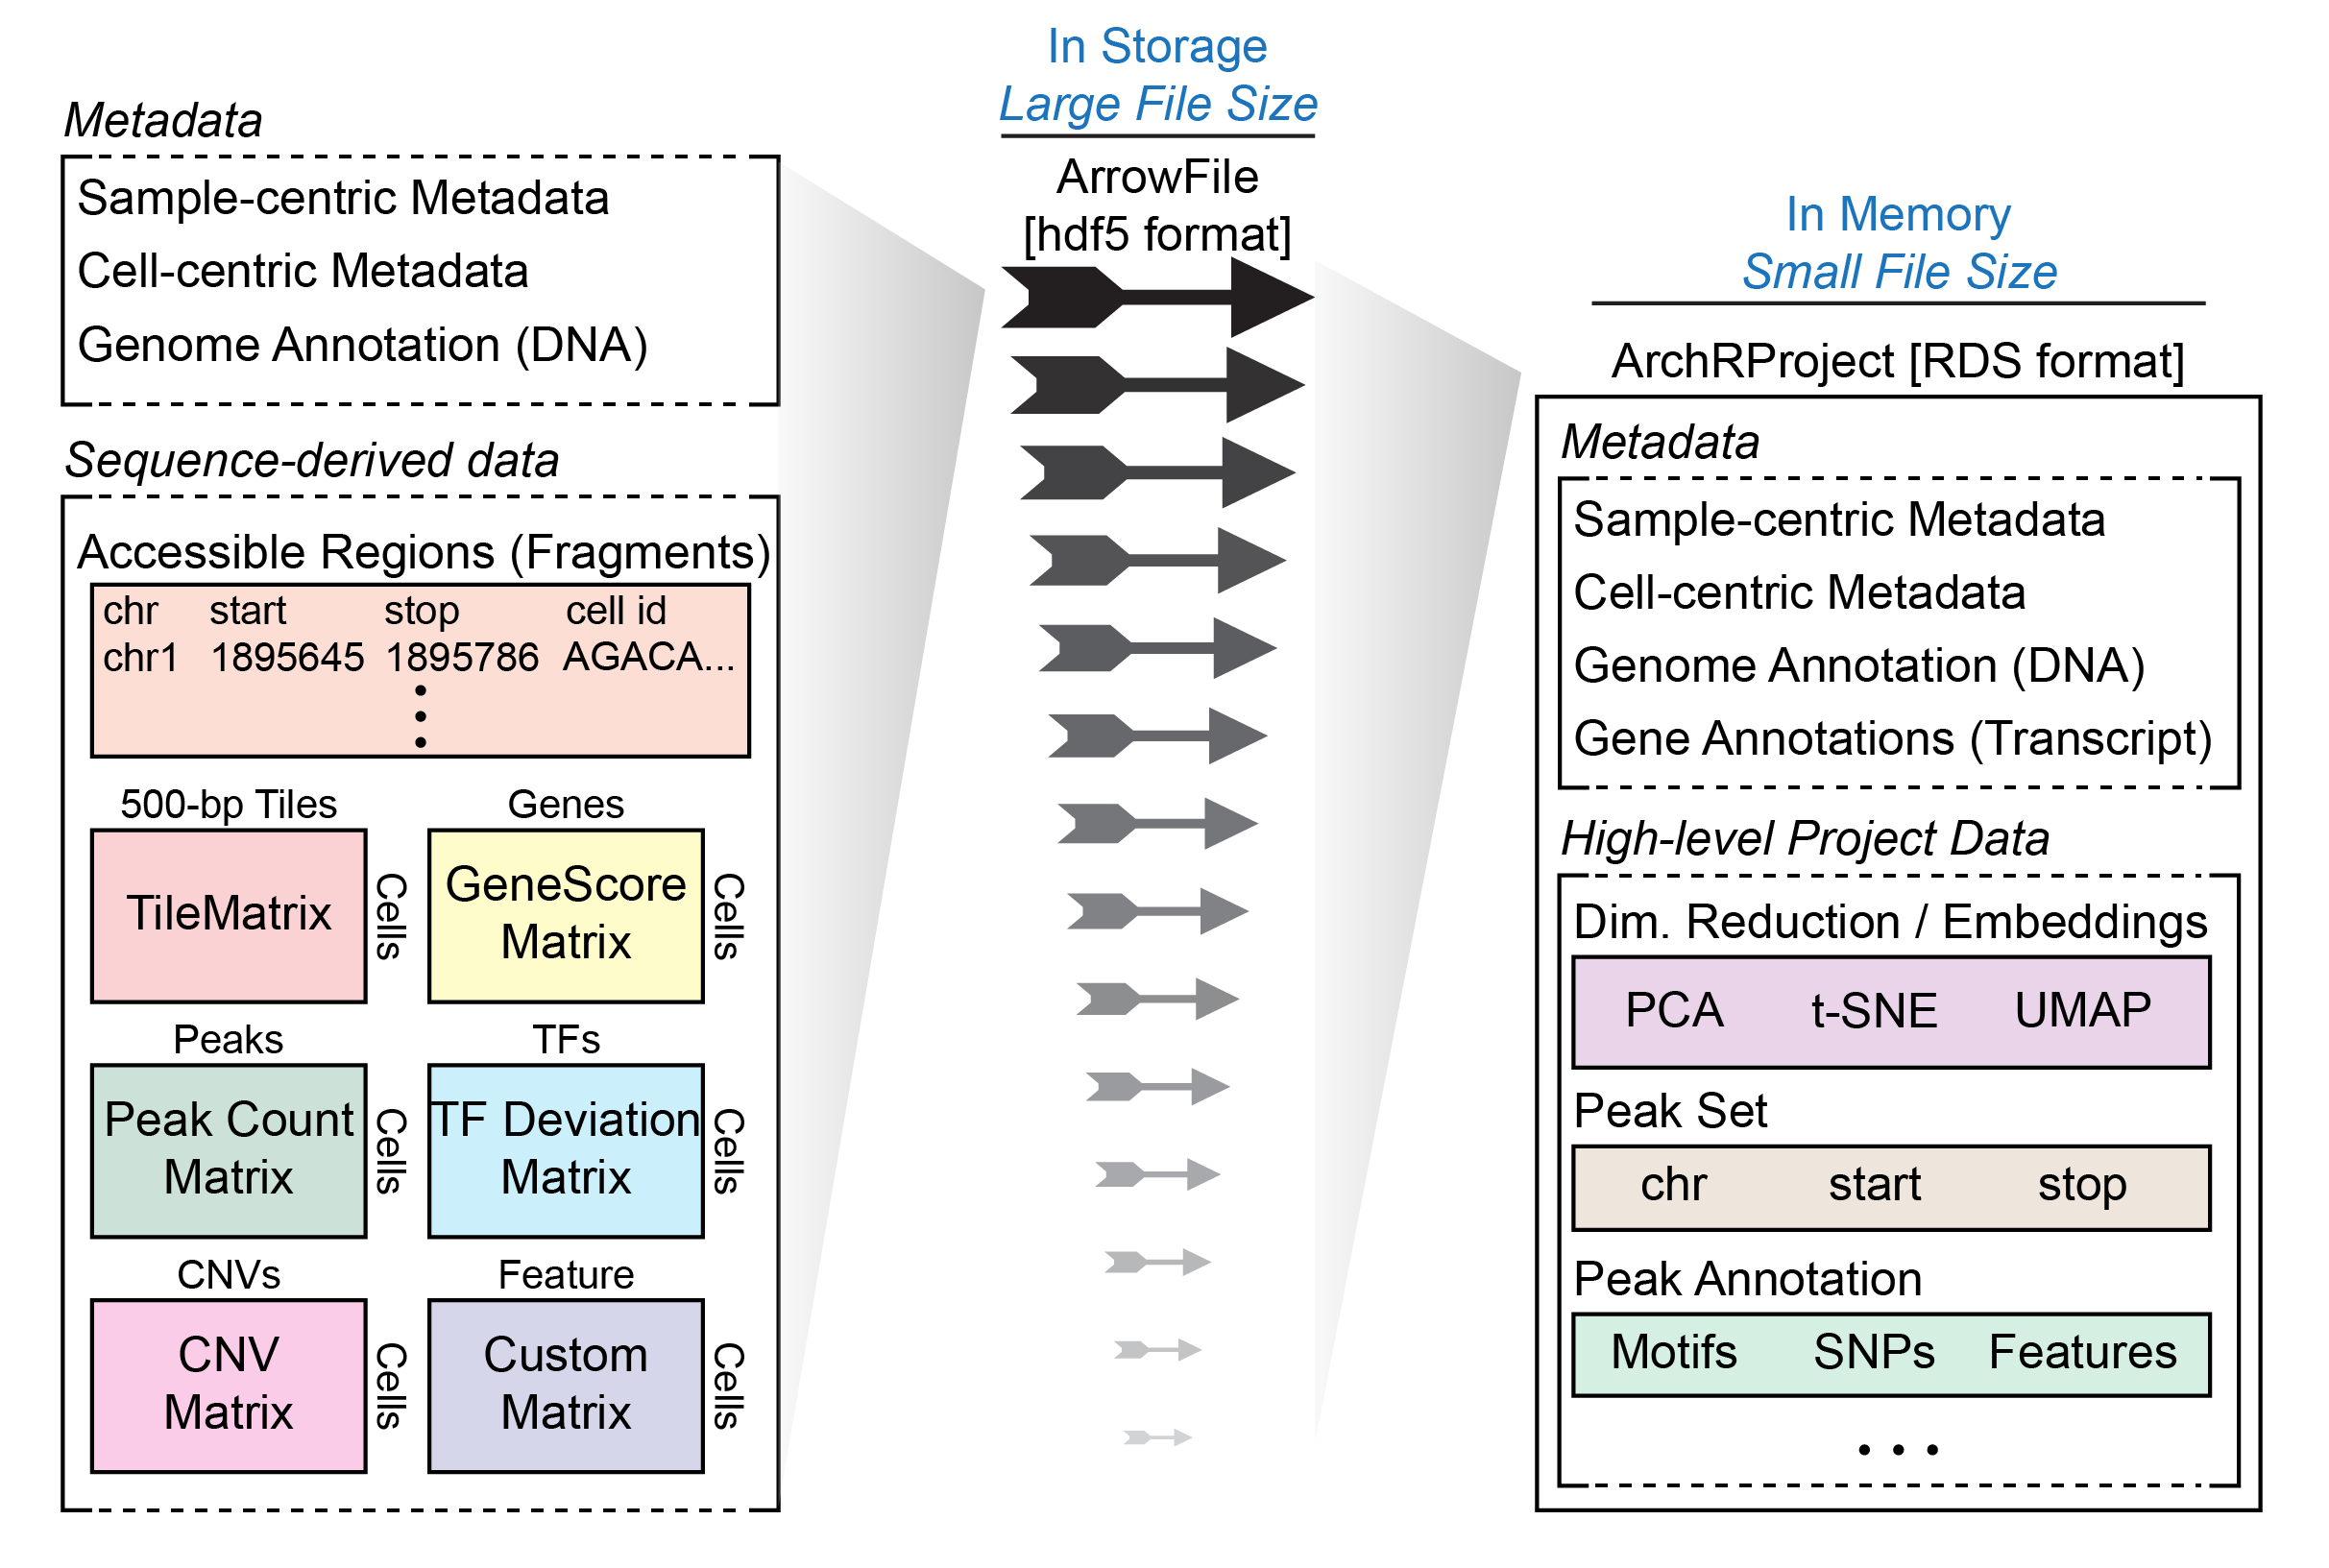
\includegraphics[width=7.29167in,height=\textheight]{images/ArchRProject_Schematic.png}

Certain actions can be taken directly on \texttt{ArrowFiles} while other actions are taken on an \texttt{ArchRProject} which in turn updates each associated \texttt{ArrowFile}. Because \texttt{ArrowFiles} are stored as large HDF5-format files, ``get-er'' functions in ArchR retrieve data by interacting with the \texttt{ArchRProject} while ``add-er'' functions either (i) add data directly to \texttt{ArrowFiles}, (ii) add data directly to an \texttt{ArchRProject}, or (iii) add data to \texttt{ArrowFiles} by interacting with an \texttt{ArchRProject}.

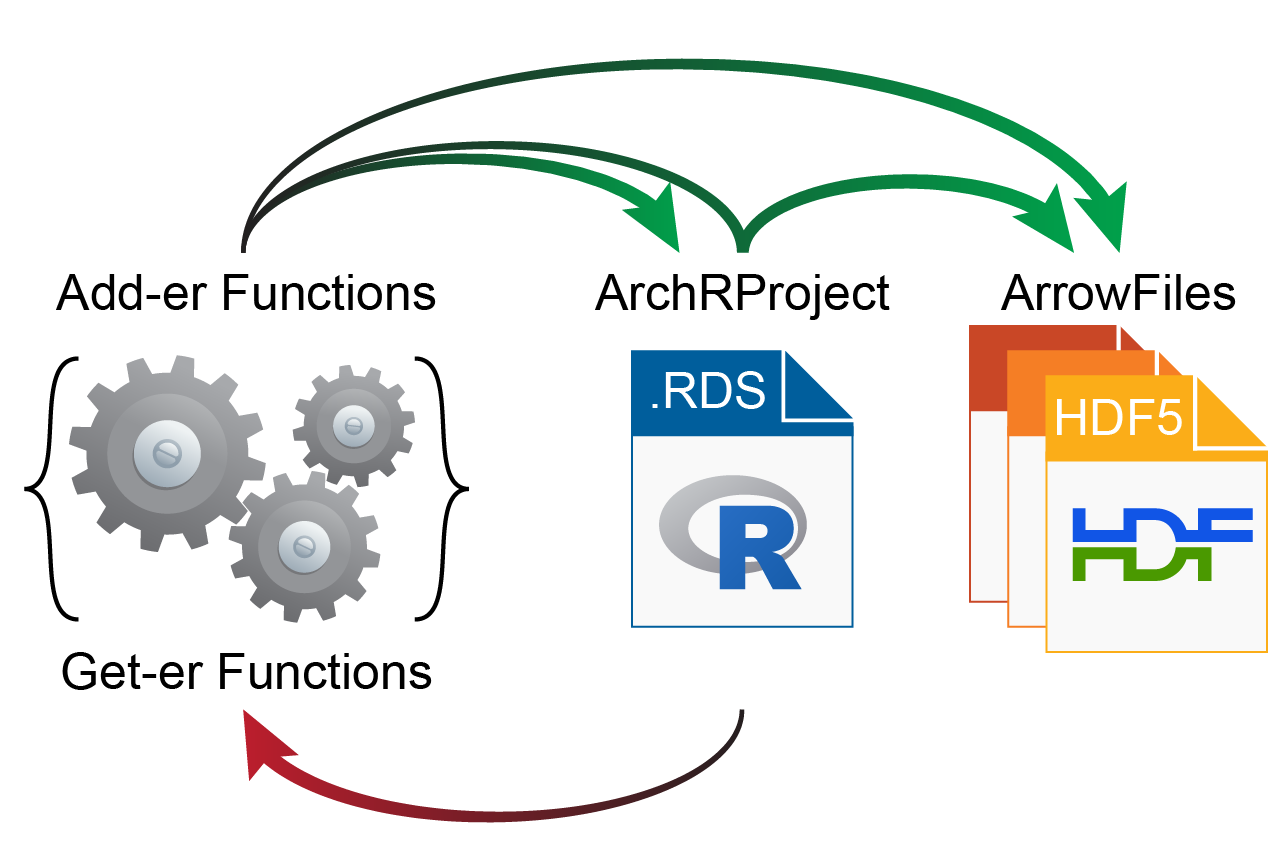
\includegraphics[width=4.16667in,height=\textheight]{images/ArchR_FunctionSchematic.png}

\hypertarget{getting-set-up}{%
\section{Getting Set Up}\label{getting-set-up}}

The first thing we do is set up our working directory, load our gene and genome annotations, and set the number of threads we would like to use. Depending on the configuration of your local environment, you may need to modify the number of \texttt{threads} used below in \texttt{addArchRThreads()}. By default ArchR uses half of the total number of \texttt{threads} available but you can adjust this manually as you see fit. If you are using windows, the usable \texttt{threads} will automatically be set to 1 because the parallel processing in ArchR is build for Unix-based operating systems.

For the purposes of this tutorial, we provide the gene and genome annotations but you can create your own using the \texttt{createGeneAnnotation()} and \texttt{createGenomeAnnotation()} functions. See the \href{articles/Articles/annotations.html}{Gene and Genome Annotations vignette} for more information.

\begin{Shaded}
\begin{Highlighting}[]
\CommentTok{\#Load R Libraries}
\KeywordTok{library}\NormalTok{(ArchR)}

\CommentTok{\#Create a new folder and set this as the working directory for tutorial analyses}
\NormalTok{wd <{-}}\StringTok{ "ArchR\_tutorial"}
\KeywordTok{dir.create}\NormalTok{(wd, }\DataTypeTok{showWarnings =} \OtherTok{FALSE}\NormalTok{, }\DataTypeTok{recursive =} \OtherTok{TRUE}\NormalTok{)}
\KeywordTok{setwd}\NormalTok{(wd)}

\CommentTok{\#Load genome annotations. Available annotations are for "Hg19", "Hg38", "Mm9", or "Mm10". QQQ THIS DOESNT MAKE SENSE. THE DATA IS HUMAN, NOT MOUSE, AND IS ONLY AVAILABLE FOR ONE GENOME FOR THE TUTORIAL? WOULD REMOVE.}
\KeywordTok{data}\NormalTok{(}\StringTok{"geneAnnoHg19"}\NormalTok{)}
\KeywordTok{data}\NormalTok{(}\StringTok{"genomeAnnoHg19"}\NormalTok{)}
\NormalTok{geneAnno <{-}}\StringTok{ }\NormalTok{geneAnnoHg19}
\NormalTok{genomeAnno <{-}}\StringTok{ }\NormalTok{genomeAnnoHg19}

\CommentTok{\#Set Default Threads for ArchR Functions}
\KeywordTok{addArchRThreads}\NormalTok{(}\DataTypeTok{threads =} \KeywordTok{floor}\NormalTok{(parallel}\OperatorTok{::}\KeywordTok{detectCores}\NormalTok{()}\OperatorTok{/}\DecValTok{2}\NormalTok{)) }\CommentTok{\#QQQ I favor including default values to make it clear what happens. Open to suggestions though.}
\end{Highlighting}
\end{Shaded}

\hypertarget{creating-arrow-files}{%
\chapter{Creating Arrow Files}\label{creating-arrow-files}}

For this tutorial, we will download a collection of fragment files. Fragment files are one of the base file types of the 10x Genomics analytical platform (and other platforms) and can be easily created from any BAM file. See \href{articles/Articles/inputFiles.html}{the ArchR input file types vignette} for information on making your own fragment files for input to ArchR. Once we have our fragment files, we provide their paths as a character vector to \texttt{createArrowFiles()}. During creation, some basic metadata and matrices are added to each \texttt{ArrowFile} including a ``TileMatrix'' containing insertion counts across genome-wide 500-bp bins (see \texttt{addTileMatrix()}) and a ``GeneScoreMatrix'' that is determined based on weighting insertion counts in tiles nearby a gene promoter (see \texttt{addGeneScoreMatrix()}). These gene activity scores are described in more depth in the \href{articles/Articles/geneScores.html}{Gene Activity Score vignette}.

\begin{Shaded}
\begin{Highlighting}[]
\CommentTok{\#Get Tutorial Data \textasciitilde{}2.2GB To Download (if downloaded already ArchR will bypass downloading).}
\NormalTok{inputFiles <{-}}\StringTok{ }\KeywordTok{getTutorialData}\NormalTok{(}\StringTok{"Hematopoiesis"}\NormalTok{)}

\CommentTok{\#Create Arrow Files (\textasciitilde{}10{-}15 minutes) w/ helpful messages displaying progress.}
\CommentTok{\#For each sample, this step will:}
\CommentTok{\# 1. Read accessible fragments.}
\CommentTok{\# 2. Calculate QC Information for each cell (TSS Enrichment, Nucleosome info).}
\CommentTok{\# 3. Filter cells based on QC parameters.}
\CommentTok{\# 4. Create a genome{-}wide TileMatrix using 500{-}bp bins.}
\CommentTok{\# 5. Create a GeneScoreMatrix using the provided geneAnnotation.}
\NormalTok{ArrowFiles <{-}}\StringTok{ }\KeywordTok{createArrowFiles}\NormalTok{(}
  \DataTypeTok{inputFiles =}\NormalTok{ inputFiles,}
  \DataTypeTok{sampleNames =} \KeywordTok{names}\NormalTok{(inputFiles),}
  \DataTypeTok{geneAnnotation =}\NormalTok{ geneAnno,}
  \DataTypeTok{genomeAnnotation =}\NormalTok{ genomeAnno,}
  \DataTypeTok{filterTSS =} \DecValTok{4}\NormalTok{,}
  \DataTypeTok{filterFrags =} \DecValTok{1000}\NormalTok{,}
  \DataTypeTok{addTileMat =} \OtherTok{TRUE}\NormalTok{,}
  \DataTypeTok{addGeneScoreMat =} \OtherTok{TRUE}
\NormalTok{  )}
\end{Highlighting}
\end{Shaded}

\begin{center}\rule{0.5\linewidth}{0.5pt}\end{center}

\hypertarget{qc-tss-scores-by-unique-fragments}{%
\section{QC TSS Scores by Unique Fragments}\label{qc-tss-scores-by-unique-fragments}}

Since this was plotted prior to creation of an ArchRProject we go to QualityControl/scATAC\_BMMC\_R2/scATAC\_BMMC\_R2-TSS\_by\_Unique\_Frags.pdf for the plot below.

\hypertarget{qc-fragment-size-distribution}{%
\section{QC Fragment Size Distribution}\label{qc-fragment-size-distribution}}

Since this was plotted prior to creation of an ArchRProject we go to QualityControl/scATAC\_BMMC\_R2/scATAC\_BMMC\_R2-Fragment\_Size\_Distribution.pdf for the plot below.



\end{document}
